\chapter{Related Work}

In the first chapter we have touched upon the history of usage of procedural generation in game creation. A comprehensive exploration of the current stage of procedural generation in games can be found in \cite{pcgbook}. In this chapter we will be more focused, exploring more closely on existing use of this technique in circumstances similar to that of our research question.

\section{Procedurally-generated game design}

First we try to contextualise TRPG battle systems within the landscape of game content generation. Hendrikx et al.\cite{hendrikx2013procedural}\ identified six levels of content, as shown in figure \ref{fig:pyramid}. Content at the bottom of the pyramid is more elementary and peripheral, whereas the upper classes are more complex entities. Under this scheme, TRPG battle systems can be classified under \textit{system design}, a part of the \textit{game design} layer within the pyramid. System design is defined as `the creation of rules and underlying mathematical patterns in a game'\cite[5]{brathwaite2009challenges}, which is definitely a fit description of TRPG battle systems.

\begin{figure}
	\centering
	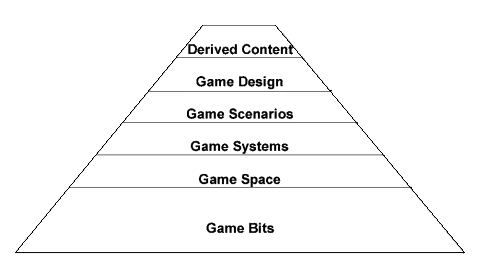
\includegraphics[width=.6\linewidth]{figures/PCG_pyramid}
	\caption{Layers of procedurally-generated game content. (adapted from \cite{hendrikx2013procedural})}
	\label{fig:pyramid}
\end{figure}

Some work does not focus on generating the game rules themselves, but rather how to combine and match the rules to concrete representations. A notable example is  \textbf{EGGG}\cite{orwant2000eggg}. This automatic programming system takes a minimal descriptive rule set of a game, written in a domain specific language, then `fleshes out' the game by using heuristics to fill in details of the rules, and packaging it as a playable game, complete with graphical user interface and an AI opponent.

Closer to our interest are works that focus on generating the whole set of rules for the games. An early example, \textbf{METAGAMER}\cite{pell1992metagame}, is a system that generates games in the class of `symmetric chess-like board games', developed  with the purpose to encourage game AI development away from being too specific to a game (such as chess) and into the direction of general game-playing. METAGAMER uses a game grammar that describes a wide range of games, and for its purposes of creating more games for the AI to play, there was no need to give preferences to any specific properties -- game instances were merely picked at random.
	
Hom and Marks\cite{hom2007automatic} extended the idea, by describing a system that also generates board games, but with a specific goal of \textit{balance}. Board games are described using Lisp-like description language originally created for \gameref{zog} -- a commercial general board game playing system, developed by Jeff Mallett and Mark Loeffler.\cite{levy2005robots} Genetic programming is then used to evolve a population of games using a fitness function that measure games balance.

The idea of using evolutionary algorithm (of which genetic algorithm / genetic programming are subtypes) to measure the quality of generated games has since become common. Ludi\cite{browne2010evolutionary} is a complete system that generates, evaluates, and creates playable user interface, using evolutionary approach. Games are described using its own general game playing description language. Rules are evolved using genetic programming, as shown in figure \ref{fig:ludi}. Standard genetic operations of crossover and mutation are applied to the population of games, then surviving games are evaluated, using a large number of criteria. The success of Ludi is proven by the fact that \gameref{yavalath}, one of the games generated from the system, has been published commercially, and was ranked in the top 100 abstract strategy board games ever invented.\cite{browne2011yavalath}

\begin{figure}
	\centering
	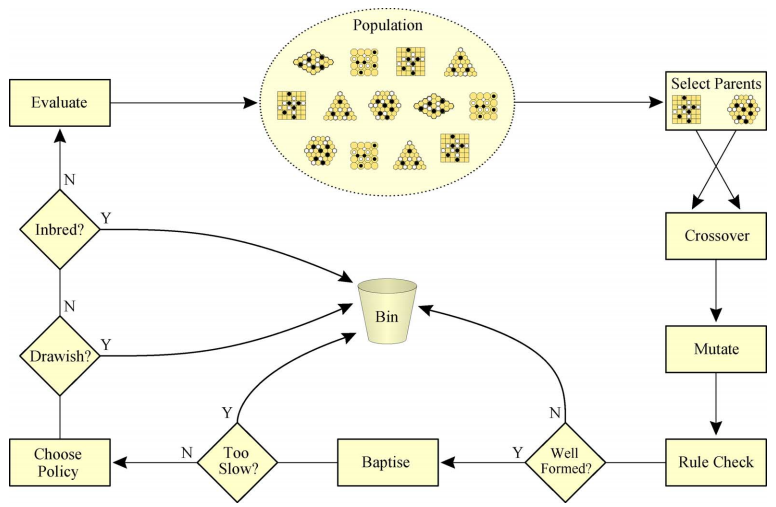
\includegraphics[width=.8\linewidth]{figures/ludi}
	\caption{Evolution process for games in Ludi system. Figure taken from \cite{browne2010evolutionary}.}
	\label{fig:ludi}
\end{figure}

\begin{figure}
	\centering
	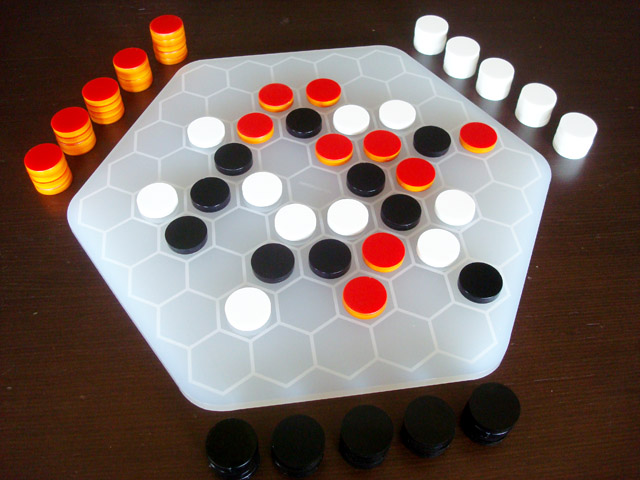
\includegraphics[width=.8\linewidth]{figures/yavalath.jpg}
	\caption{\textit{Yavalath}, a commercial game generated from Ludi.}
	\label{fig:yavalath}
\end{figure}

Progress has also been made on generating game rules for graphical video games. An experimental system by Togelius and Schmidhuber\cite{togelius2008experiment} was able to generate discrete, Pacman-like games, also by using evolutionary algorithm. Variations Forever\cite{smith2010variations} instead uses \textit{answer set programming}, a form of logic programming, to generate rule sets of graphical 2-D video games that satisfy given constraints, without using evaluation function. In the same manner that game description languages, originally created for general game-playing AI development, have been used to evolve abstract board games, Video Game Description Language (VGDL)\cite{ebner2013towards}, which was proposed to assist in \textit{general video game playing}, could also be exploited to generate video games.

Similar efforts to extend or create game description languages have been done on several other domains, and therefore can also be used for game generation. These includes card games\cite{font7835card}, action-adventure games\cite{dormans2012generating}, puzzles\cite{web-puzzlescript}, general real-time games\cite{kowalski15game}, and strategy games\cite{mahlmann2011towards}.
	
\section{Procedural generation in strategy games}

To the best of our knowledge, procedural generation has never been attempted in the specific case of TRPG battle systems. However, works in related genres exist. In one sense, TRPG battles can be thought of as more complex board games, which have been a primary subject of procedural generation research, as already presented in the previous section. In another perspective, TRPG battles are very similar to turn-based strategy games. There exists research in using procedural generation on strategy games, though not as extensive as in board games.

Some of these works\cites{togelius2010multiobjective, liapis2013generating} focus on the task of \textit{map generation} in games such as \gameref{starcraft}. Maps play a big role in strategy games in general, since the positions of resources required for various activities do influence how the game might progress. In contrast, such resources usually do not exist in TRPG, and while TRPG battle maps do affect the positioning of units, which in turn could affect the effectiveness of units' skills, they are not as influential.

Another work by Mahlmann et al.\cite{mahlmann2011towards}\ explores the balance of units in turn-based strategy games. First they developed the Strategy Game Description Language (SGDL) to describe a landscape of strategy games, then developed an AI that is able to play any games defined in SGDL, and use genetic programming to create a balanced set of units for a simplistic strategy game. The fitness function used in the evolution was based on the damage each type of unit can inflict upon each other. Based on this successful result, if SGDL is extended further to include other aspects of strategy games, then it could be possible to automatically generate all aspects of this type of games.

\section{Discussion}

In this chapter we have looked into the attempts to use procedural generation techniques to create game content at a level similar to that of TRPG battle systems. Search-based procedural generation techniques -- in particular evolutionary programming with simulation-based fitness function -- are common, since evaluation of the generated content at the level of game rules and mechanics is difficult (or impossible) to achieve without actually experiencing the games in some way.\cite{togelius2010search} A number of these systems operate at a level above any specific game, using a game description language to describe a large set of games. Game rules have been generated for different domains, such as abstract board games, graphical 2-D video games, and, most interesting for our purposes, strategy games.

For the scope of this work, we will focus on a single prototypical game as a representation of TRPG battles, therefore a game description language is not needed. Evolutionary algorithm, however, appears to be a successful paradigm for this kind of task, and therefore would be adopted as our main approach to the solution of our research question, the design of which will be explored in the next chapter.